%%%%%%%%%%%%%%%%%%%%%%%%%%%%%%%%%%%%%%%%%
% University/School Laboratory Report
% LaTeX Template
% Version 3.1 (25/3/14)
%
% This template has been downloaded from:
% http://www.LaTeXTemplates.com
%
% Original author:
% Linux and Unix Users Group at Virginia Tech Wiki 
% (https://vtluug.org/wiki/Example_LaTeX_chem_lab_report)
%
% License:
% CC BY-NC-SA 3.0 (http://creativecommons.org/licenses/by-nc-sa/3.0/)
%
%%%%%%%%%%%%%%%%%%%%%%%%%%%%%%%%%%%%%%%%%

%----------------------------------------------------------------------------------------
%	PACKAGES AND DOCUMENT CONFIGURATIONS
%----------------------------------------------------------------------------------------

\documentclass[12pt]{report}

\usepackage{graphicx} % Required for the inclusion of images
\usepackage{hyperref}
\usepackage{amsmath} % Required for some math elements 
\usepackage{indentfirst}
\usepackage{xcolor}
\usepackage{caption}
\usepackage{listings}
\usepackage{biblatex}
\usepackage[margin=1.0in]{geometry}

\setlength\parindent{0pt} % Removes all indentation from paragraphs

\hypersetup{
	colorlinks=true,
	linkcolor=blue,
	filecolor=magenta,
	urlcolor=blue,
}
\definecolor{dkgreen}{rgb}{0,0.6,0}
\definecolor{ltgray}{rgb}{0.5,0.5,0.5}

\DeclareCaptionFont{white}{\color{white!50}}
\DeclareCaptionFormat{listing}{\hspace{-3pt}\colorbox{gray}{\parbox{\textwidth}{#1#2#3}}}
\captionsetup[lstlisting]{format=listing,labelfont=white,textfont=white}

\newif\ifcolname
\colnamefalse


%%% https://tex.stackexchange.com/questions/455993/formatting-sql-code
\definecolor{codegreen}{rgb}{0,0.6,0}
\definecolor{codegray}{rgb}{0.5,0.5,0.5}
\definecolor{codepurple}{HTML}{C42043}
\definecolor{backcolour}{HTML}{F2F2F2}
\definecolor{bookColor}{cmyk}{0,0,0,0.90}  
\color{bookColor}

\lstset{
	language=sql,
	basicstyle=\ttfamily,
	showspaces=true,
	upquote=true,
	}

\lstdefinestyle{mystyle}{
	backgroundcolor=\color{backcolour},   
	commentstyle=\color{codegreen},
	keywordstyle=\color{codepurple},
	numberstyle=\numberstyle,
	stringstyle=\color{codepurple},
	basicstyle=\footnotesize\ttfamily,
	breakatwhitespace=false,
	breaklines=true,
	captionpos=b,
	keepspaces=true,
	numbers=left,
	numbersep=10pt,
	showspaces=false,
	showstringspaces=false,
	showtabs=false,
}
\lstset{style=mystyle}

%%%%%%%%%%

\renewcommand{\baselinestretch}{1.2}
\addbibresource{sample.bib}
%----------------------------------------------------------------------------------------
%	DOCUMENT INFORMATION
%----------------------------------------------------------------------------------------

\title{ A Brief on Asteroids for\\ Potential Mining\\ CSCI 403} % Title

\author{Jacob \textsc{Mcbee}} % Author name

\date{May 3, 2021} % Date for the report

\begin{document}

\maketitle % Insert the title, author and date


%----------------------------------------------------------------------------------------
%	SECTION Intro
%----------------------------------------------------------------------------------------

\section*{Introduction}
\;\;\;\; Our solar system is rich, hoarding vast resources that are constantly out of reach. While on Earth we believe our stockpiles to be plentiful for the near future, hopeful for the long term, we are missing an opportunity of grandeur just within a couple years of travel time. Asteroids, long thought to be remnants of failed protoplanets, may host the answer to a never ending supply of resources and materials needed for the modern world. At least, this is speculated on initial surveying, and there have been previous attempts by various startup companies aiming for the prize. But the companies all stopped, coming to similar conclusions of infeasibility. What exactly were they looking at when they made these conclusions, and exactly how many resources can we approximate there to be? 


\section*{Dataset}
\;\;\;\; This project used a dataset found on \hyperlink{https://www.kaggle.com/sakhawat18/asteroid-dataset}{kaggle} under Open Data Commons Open Database License [\cite{Hossain}]. The original source of the data comes from NASA's Asteroid Data Set [\cite{JPL}]. The dataset comes in CSV format, and is all contained within a single table, of which has many attributes. Many of these attributes are for identification purposes, such as the given name for an asteroid (the largest known asteroid, Ceres, is listed with its given name) or even ID numbers for different systems. The rest of the data is all measurements taken on the asteroids, containing useful information such as the diameter of the asteroid, the distance from the Sun, and the possibility of potential hazards. 

\;\;\;\; To answer our question of how much can be mined from asteroids, we want to find out how much raw material there approximately is in our solar system. Some large assumptions are made -- such as asteroids being spherical, as the data is plenty and the measurements can only be so precise without tools directly on an asteroid's surface. Luckily, the single most important attribute for determining composition of an asteroid is its albedo. This attribute tells us the reflectivity of an asteroid's surface, which is used when classifying asteroids into various groupings. These groupings will be our new tables filtered down from our large dataset into smaller concise ones for easier reading. 

\;\;\;\; Our other question, why did companies who considered planning to mine asteroids stop operations, will be assumed to be due to costs of operations only, and not lack of a plan. For this, we will only assume a fix cost based only on various statistics related to current costs of spaceflight reported by either private companies or NASA, and using the distances to asteroids from our dataset to determine overall cost. Then, by combining the results of our approximation of resources and the overall predicted cost to gather resources, we can find an answer as to why no one is attempting to mine asteroids.

%----------------------------------------------------------------------------------------
%	SECTION 2
%----------------------------------------------------------------------------------------

\thispagestyle{empty}
\section*{Initialization Code}
The following code is the setup for creating and filtering data into more easily usable tables. First is actually creating a database and schema to read in the dataset. This was done on a private machine and not a public database, just for ease of access.

\hspace{-1.6cm}
\begin{lstlisting}{language=sql, deletekeywords={IDENTITY},deletekeywords={[2]INT},morekeywords={clustered},framesep=8pt,xleftmargin=40pt,framexleftmargin=40pt,frame=tb,	framerule=0pt}
CREATE DATABASE asteroids WITH ENCODING 'UTF8' 
	LC_COLLATE='en_US.UTF-8' 		
	LC_CTYPE='en_US.UTF-8';
GRANT TEMP ON DATABASE asteroids TO public;
GRANT SELECT, INSERT, UPDATE, DELETE ON ALL TABLES IN SCHEMA public TO public;
GRANT EXECUTE ON ALL FUNCTIONS IN SCHEMA public TO public;
GRANT USAGE ON ALL SEQUENCES IN SCHEMA public TO public;

DROP TABLE IF EXISTS asteroid_data;
CREATE TABLE asteroid_data (
	id VARCHAR(1024),
	spkid SERIAL,
	full_name VARCHAR(255),
	pdes VARCHAR(50),
	name VARCHAR(255),
	prefix VARCHAR(1),
	neo BOOLEAN,
	pha BOOLEAN,
	H FLOAT,
	diameter FLOAT,
	albedo FLOAT,
	...
	sigma_per FLOAT,
	class VARCHAR(50),
	rms FLOAT,
	PRIMARY KEY (spkid)
)\end{lstlisting}


From here, we can filter out the data into groupings of asteroids based on their albedo characteristic. We want to add other useful attributes to answer other questions later. 


The composition breakdown of asteroids is currently unknown, however we can approximate from meteorites that have fallen to Earth a basic breakdown. For the purposes of simplifying the report, we are only interested in the most common types of materials. In our case, C-Types have carbon, S-Types have silicon, M-Types have various heavy metals, such as iron, platinum, or nickel [\cite{Rivkin}]. The precise numbers vary wildly from a 40\%-70\% composition of these main materials, and so we will assume a lower bound, that 20\% of the asteroid's volume is the materials we want. For now, we separate the albedo's into their own tables for ease later.

\thispagestyle{empty}


\begin{lstlisting}[language=sql, deletekeywords={IDENTITY},
		deletekeywords={[2]INT},
		morekeywords={clustered},
		framesep=8pt,
		xleftmargin=40pt,
		framexleftmargin=40pt,
		frame=tb,
		framerule=0pt]
\copy aseteroid_data from dataset.csv csv header;

-- Find probable C-type Asteroids
-- These are mostly carbonous and the most common

SELECT id, diameter, a as semi_major, q as perihelion 
INTO TABLE c_type
FROM asteroid_data
WHERE albedo <= 0.10;

-- Find probable M-type Asteroids

SELECT id, diameter, a as semi_major, q as perihelion 
INTO TABLE m_type
FROM asteroid_data
WHERE albedo > 0.10 AND albedo < 0.20;

-- Find probable S-type Asteroids

SELECT id, diameter, a as semi_major, q as perihelion 
INTO TABLE s_type
FROM asteroid_data
WHERE albedo >= 0.20;
\end{lstlisting}

These type designations are used in determining the material composition of asteroids, as the reflective surface of a given body usually will indicate the most abundant raw material on a body [\cite{ORourke}]. For this project, only the diameter, semi major axis, and perihelion will be used. The diameter will be used in approximating the volume of a given asteroid so we can tell how many resources may be obtained from them. The semi major and perihelion can both be used to gauge a distance from the sun and find out how far from Earth they are. That last part becomes important in understanding why the space mining companies stopped their operations.

%----------------------------------------------------------------------------------------
%	SECTION 3
%----------------------------------------------------------------------------------------

\newpage
\section*{Data Collecting}
\;\;\;\; After initializing and filtering the data, we can start collecting some useful information on the reduced dataset. For plotting the data, python and the matplotlib library was used. The first thing we want to look for are the total counts of known asteroids versus unknown. The SQL code is included in the end of the report.

\begin{center}
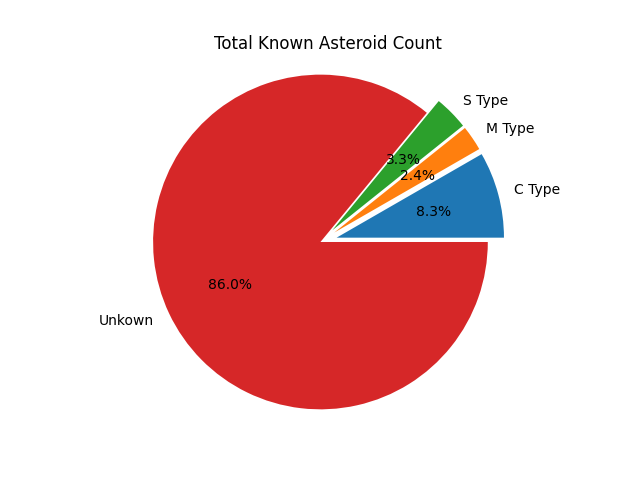
\includegraphics[scale=0.6]{"charts/total_counts.png"}
\end{center}

As shown, most of the asteroids are of unknown type, meaning there is no albedo listed. This is probably due to measurements being uncertain and the asteroid being too small to accurately tell the albedo. To find out, we can instead run a similar query to find the types of asteroids based on their assumed volume.

\begin{center}
	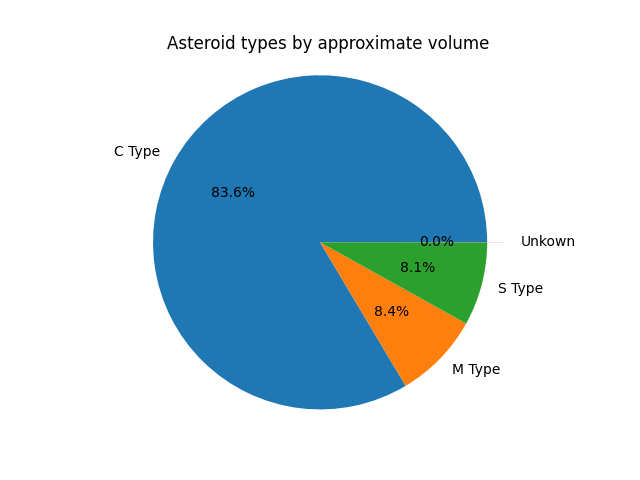
\includegraphics[scale=0.6]{"charts/approx_vol.png"}
\end{center}

\;\;\;\; Now we can see that the majority of asteroids by volume have indeed been identified. Perhaps important to note, that various ideas of mining asteroids involve moving asteroids closer to Earth for mining operations, in this case the unknown asteroids would be the most likely candidates for moving since they are by far the smallest. We do not assume that is an issue though as we only want to find the total amount of material. From this point forward, we ignore the unknown types since their total volume would be insignificant. 

\;\;\;\; Now we grab the assumed total volume of the various asteroid types and apply our lower bound set earlier of 20\% usable material. More assumptions are made in the densities to calculate the final weights, but they the asteroids are assumed to be approximately uniform in weight and distributions. Shown below is the calculated masses of all materials and the entire mass of Earth.

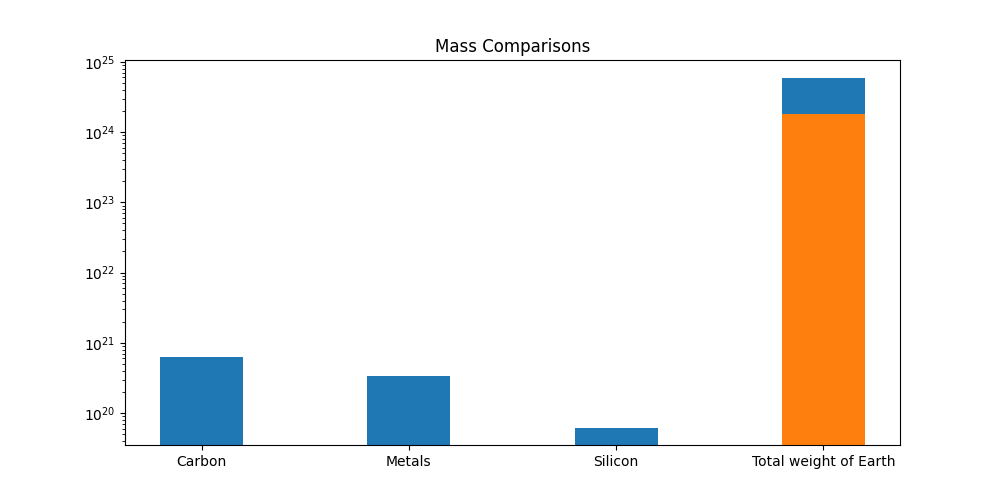
\includegraphics[scale=0.7]{"charts/mass.png"}

\;\;\;\; Shown on the total mass of the Earth is the projected amount of raw silicon on Earth. About 27\% of the mass of Earth is silicon, and there are similar numbers for our metals and carbon combined. However, it is important to note that the majority of these on Earth materials are difficult to reach, as much of it is under the oceans, lie underneath mountains, and is included in areas where people already live. In addition, these resources can be hundreds of kilometers below the surface, meaning a vast majority of it will be unobtainable for the foreseeable future [\cite{Sharp}]. 

\;\;\;\; It would be better to look at how much was actually mined on Earth in recent years. In one estimate, China, the world leader in silicon exportation and mining, had mined up to approximately 4.5 million metric tons of silicon in 2019, or 4.5 billion kg and accounted for $\frac{2}{3}$ of all silicon mining [\cite{Statista}]. Our lower bound approximation is about $10^{11}$ times the amount of the annual mined material, thus indicated that there are unimaginable resources available.
%----------------------------------------------------------------------------------------
%	SECTION 4
%----------------------------------------------------------------------------------------
\section*{Why did they stop?}

\;\;\;\; So if there are so many resources, beyond what we will ever be able to produce on Earth, why don't companies take the plunge? Or rather, why have they discontinued their ventures? Various start up companies and their CEO's looked to become what was believed to be the first trillionaires, as they all understood what was waiting. The first couple to come out, Planetary Resources, Deep Space Industries, and even NASA, all pulled out before long. The simple answer: space is really really big [\cite{PhysWorld}]. 

\includegraphics[scale=0.7]{"charts/polar.png"}

\;\;\;\; The polar plot from the last page showcases the absolute insane distances to acquire these potential resources. The Earth and Sun are only plotted to gauge distances and are not to scale, where as the asteroids are shown to scale (if possible, you can zoom in to see very small dots near Earth). Their relative angles are only randomly generated to since their positions are always changing, but virtually all asteroids are located around 2.0 to 3.0 AU's from the Sun, in other words, they are at least twice as far away from the Sun as the Earth is. This is a problem, Mars itself is already a staggering 1.5 AU's from the Sun, and traveling there with current technology is suspected to take at least 8 months one-way. Traveling to these clusters of asteroid belts would take with the same technology about 2 years one-way. Not only this, but the dispersion around the polar graph is partially to show that even if you were to go 2.5 AU's out, you would likely only reach one asteroid and the next nearest would still take days to reach. In other words, if you reached one asteroid, to reach the other thousands of known asteroids in the same $\frac{1}{8}$ region would take approximately 3 years without considering mining operations or asteroid transportation, and only if they all lied in a straight arc.

\;\;\;\; Using NASA's estimate for spacefaring costs as a mission to Mars being about \$2.7Bn, and Mars being at best 0.5 AU away from Earth, a mission to the largest Asteroid, Ceres, would take approximately \$15Bn, for our largest mining opportunity. Given this, what is the expected return? Well while no asteroid's composition is known entirely, relying only on our earlier assumptions and realizing Ceres has the most abundance of carbon, not a particularly expensive resource, has approximately \$2.38 $\times 10^{19}$ worth of material, or 20 quintillion dollars worth of carbon. Clearly, this would be so overwhelming, and the economics back on Earth would not really be prepared to handle it, but more importantly, we see that the return on investment would be beyond covered. And this idea of trillionaires is completely squashed assuming the value of the resources did not adjust according to economic theories.
%----------------------------------------------------------------------------------------
%	SECTION 5
%----------------------------------------------------------------------------------------
\newpage
\section*{Conclusions}
\;\;\;\; The dataset and gathering were both made relatively simple from kaggle and NASA, and there are more interesting columns that were completely neglected in hopes of an efficient explanation to something that has interested me for a long time. While we are still far away from potentially mining asteroids, it seems inevitably a sure thing as long as there is money and people have needs. If given enough time, I would have liked to been able to discuss Near Earth Objects or NEO's which are asteroids that are believed to be the first in mining. None of them come close to the scale of those around the asteroid belt, but they will be an important beginning to space mining. 

%----------------------------------------------------------------------------------------
%	SECTION 6
%----------------------------------------------------------------------------------------
\newpage
\section*{Data Collecting Code}

\begin{lstlisting}[language=sql, deletekeywords={IDENTITY},
	deletekeywords={[2]INT},
	morekeywords={clustered},
	framesep=8pt,
	xleftmargin=40pt,
	framexleftmargin=40pt,
	frame=tb,
	framerule=0pt]
-- General counts of likely asteroids types

SELECT *, (a_data - c_type - m_type - s_type) AS unkown 
FROM (
	SELECT 
	(
	SELECT count(*)
	FROM c_type
	)   AS c_type,
	
	(
	SELECT count(*) 
	FROM m_type
	)   AS m_type,
	
	(
	SELECT count(*)
	FROM s_type
	)   AS s_type,
	
	(
	SELECT count(*)
	FROM asteroid_data
	)   AS a_data
) AS a;

	
\end{lstlisting}

Output: 

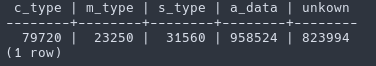
\includegraphics{"charts/q1.png"}

\newpage
\begin{lstlisting}[language=sql, deletekeywords={IDENTITY},
	deletekeywords={[2]INT},
	morekeywords={clustered},
	framesep=8pt,
	xleftmargin=40pt,
	framexleftmargin=40pt,
	frame=tb,
	framerule=0pt]
SELECT 
-- c_type approx volume in km^3
(
SELECT SUM(4*PI()*POWER((diameter/2),3)/3)
FROM c_type
)   AS volume_c,

-- m_type approx volume in km^3
(   
SELECT SUM(4*PI()*POWER((diameter/2),3)/3)
FROM m_type
)   AS volume_m,

-- s_type approx volume in km^3
(
SELECT SUM(4*PI()*POWER((diameter/2),3)/3)
FROM s_type
)   AS volume_s,

-- remaining volume of unkown type
(        
SELECT SUM(4*PI()*POWER((diameter/2),3)/3)
FROM unkown
)   AS volume_u
\end{lstlisting}

Output: 

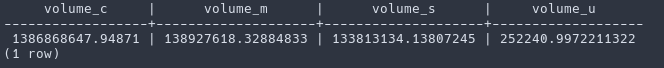
\includegraphics[scale=0.7]{"charts/q2.png"}

\begin{lstlisting}[language=sql, deletekeywords={IDENTITY},
	deletekeywords={[2]INT},
	morekeywords={clustered},
	framesep=8pt,
	xleftmargin=40pt,
	framexleftmargin=40pt,
	frame=tb,
	framerule=0pt]
-- Getting distances from the sun and diameters for plotting
-- limited to 3 AU's to be more visable

SELECT diameter, semi_major
FROM c_type
WHERE semi_major < 3 AND diameter IS NOT NULL;
	   
SELECT diameter, semi_major
FROM m_type
WHERE semi_major < 3 AND diameter IS NOT NULL;

SELECT diameter, semi_major
FROM s_type
WHERE semi_major < 3 AND diameter IS NOT NULL;
\end{lstlisting}

\newpage
\begin{lstlisting}[language=sql, deletekeywords={IDENTITY},
	deletekeywords={[2]INT},
	morekeywords={clustered},
	framesep=8pt,
	xleftmargin=40pt,
	framexleftmargin=40pt,
	frame=tb,
	framerule=0pt]
-- Approximating the amount of equivilent money Ceres could be worth
-- 0.122 is the cost of carbon $USD/kg
-- 0.2 is lower bound guess for amount of carbon
SELECT 4*PI()*POWER((diameter/2),3)/3*1000000000*0.122*0.2 AS carbon_money
FROM asteroid_data
WHERE name LIKE '%Ceres%';
\end{lstlisting}

Output:

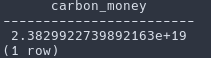
\includegraphics{"charts/q3.png"}
%----------------------------------------------------------------------------------------
%	BIBLIOGRAPHY
%----------------------------------------------------------------------------------------
\newpage

\printbibliography

%----------------------------------------------------------------------------------------


\end{document}